\documentclass[a4paper]{scrreprt}
\usepackage{etex}
\usepackage[utf8]{inputenc}
%\usepackage[T1]{fontenc}
\usepackage{lmodern}
\usepackage{hyphsubst}
\usepackage[english]{babel}
\usepackage{textcomp}
\usepackage{enumerate}
\usepackage{microtype}
\usepackage{listings}
\usepackage{graphicx}
\usepackage{subcaption}
\usepackage{titling}
\usepackage{amsmath}
\usepackage{float}
\lstset{language=[LaTeX]TeX}

\usepackage{wallpaper}

\renewcommand{\quote}[1]{``#1''}

\begin{document}
\URCornerWallPaper{0.25}{TUHH.png}
\title{Report on Exam Task\\Simulation and Modelling of Communication Networks}
\author{Nicolás Chopitea Kober, Sebastian Lindner}
\date{Summer Term 2016}
\maketitle	

\tableofcontents
\newpage

\chapter{Overview}
\section{Description}
	We were tasked by a university to analyze the usefulness, practicability and limitations of a remote university building's direct radio link to the main university campus. 
	
	In this chapter we will attempt to fully capture the scenario at hand, abstract it into a model and extract the requirements that have to be fulfilled in order to have an applicable solution to connecting the remote building with the main campus via radio.
\section{Requirement Analysis}
	\subsection{Network Description}
		The aim is to connect a remote building's network to the main university campus network. The fast cabled connection is endangered due to a construction site in close proximity to the building. That is why a direct radio link could be employed to maintain connectivity throughout the construction process.
		
		The following network usage cases could be identified:
		
		\begin{description}
		\item[CCTV] A CCTV camera is connected to the remote building's router. \\ It is continuously transmitting a livestream of its video.
		
		\item[Wireless] A wireless access point operating on the \emph{802.11g} standard is connected to the remote building's router. \\Connected to this access point are users engaged in the following three activities.
		\begin{description}
			\item[FTP Upload] A single file upload can be observed that is ongoing throughout the simulation of the network.
			\item[Video Livestream] A remotely located professor is livestreaming his or her lecture to a video conference laptop. \\This connection is bidirectional so that participating students can ask questions.
			\item[Web Browsing] A variable number of students browsing the web is connected to the access point at any time.
		\end{description}
		\end{description}
		
		This describes the network inside the remote building that we are trying to connect. The main campus' network can currently be simplified to three connections:
		
		\begin{description}
			\item[Remote Professor] A fast connection to the remotely located professor's laptop is established via the Deutsches Forschungsnetz. \\It will communicate with the video conference laptop inside the remote building.
			\item[Porter's Office] A CCTV monitoring station sits in the porter's office. \\The livestream of the remote building's CCTV camera will travel here.
			\item[Internet] A VDSL connection to the Internet is present. \\Both web browsing and FTP upload traffic will have this destination.
		\end{description}
		
		A graphical representation of the scenario is as follows and includes technical details such as channel delay and bandwidth:
		
		\begin{figure}[H]
		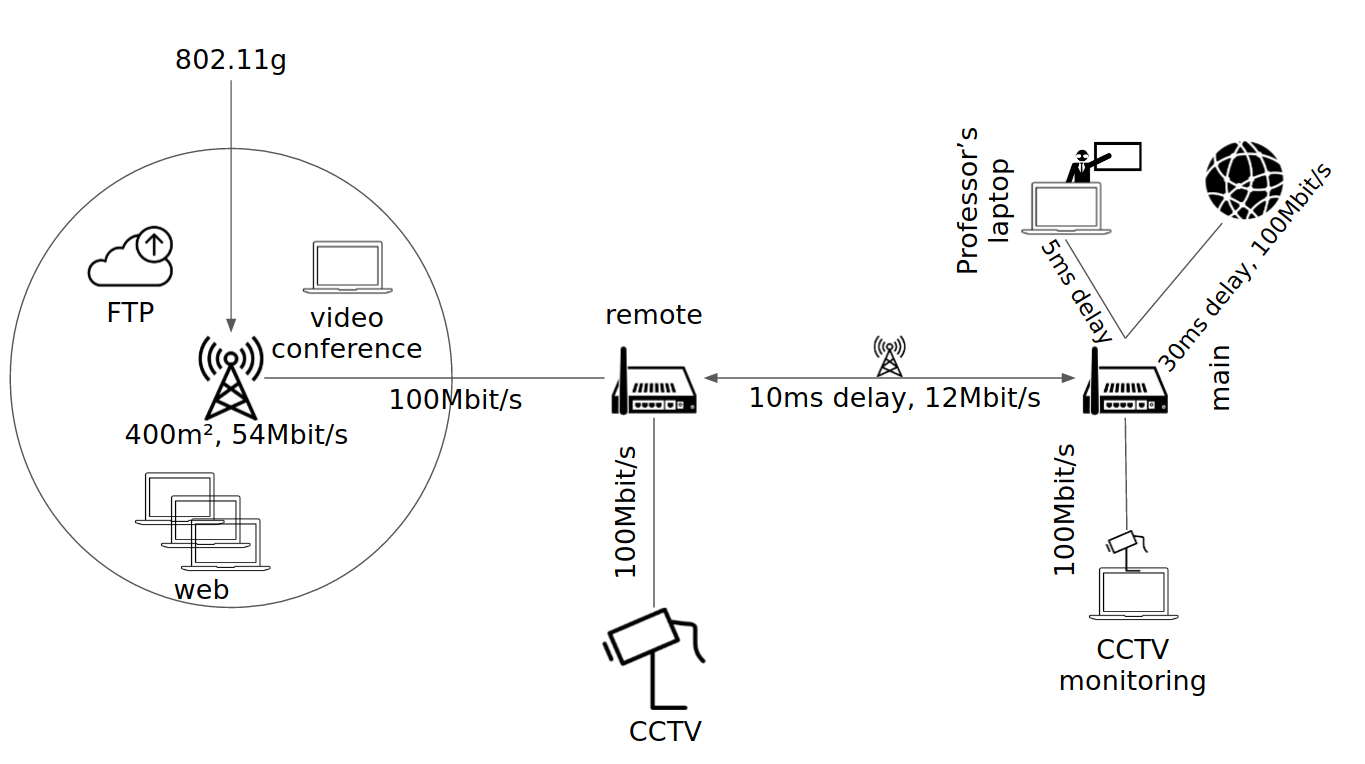
\includegraphics[width=\textwidth]{./simmodel.png}
		\caption{A model of the scenario depicted}
		\end{figure}
	\subsection{Statistical Web Browsing Model}
		The student's web browsing behavior is difficult to capture. We are going to model it by assuming a student issues an HTTP request, receives a response and then spends some time reading the response that is exponentially distributed. Missing at this point is the size of the response that follows a request. To model this we have analyzed a trace file containing 1000 response size values.
		
		We have chosen the \emph{chi squared goodness of fit test} to evaluate how well a distribution fits the observed data. As a first step we investigated the density of values within request size intervals. These intervals initially were of equal size and the observed values were associated to an interval that they lied in. To remove intervals with no values associated to them, these were merged with neighboring intervals. In this way we obtained 160 intervals of which most have observed values associated to them. This is a graphical representation of what we found:
		\begin{figure}[H]
		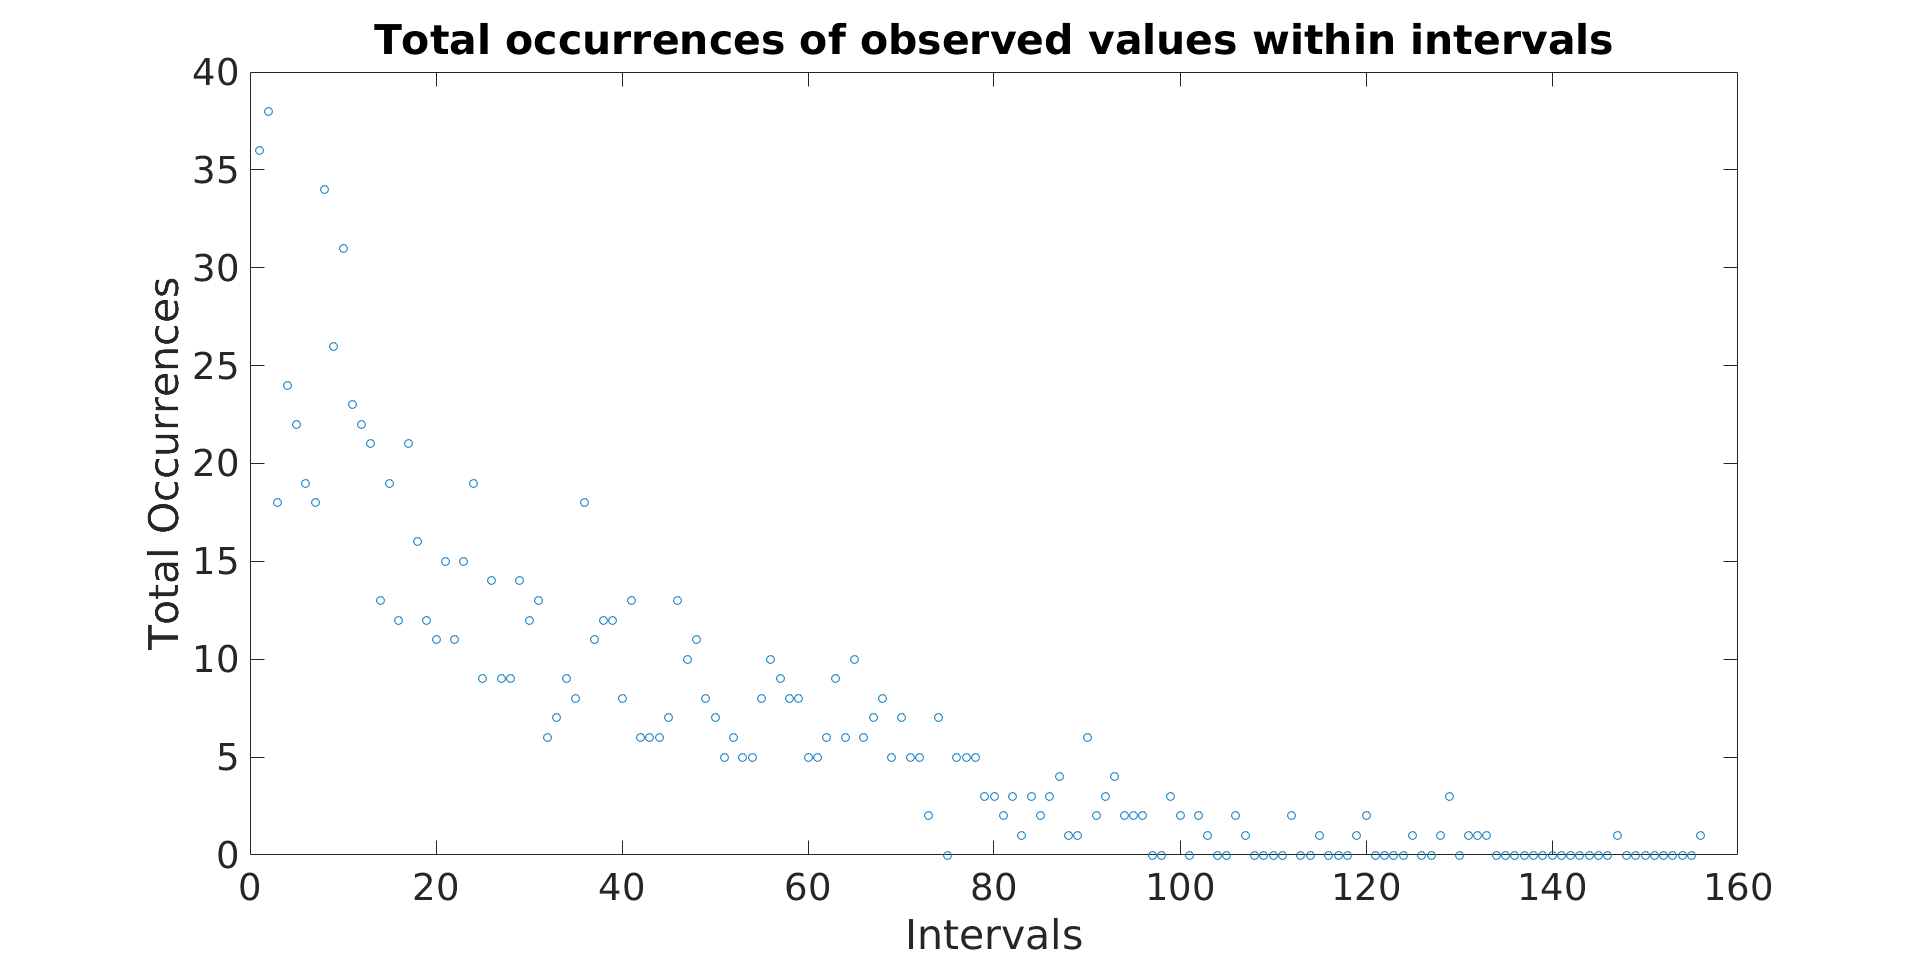
\includegraphics[width=\textwidth]{../tracefile_analysis/exp.png}
		\caption{Request size value density in intervals}
		\end{figure}
		
		We have the highest density of observed values in regions of low response sizes, and the number of observations decreases exponentially for increasing response sizes. This looks closely related to values coming from a \emph{negative exponential distribution}, which is why we decided to apply the test against this distribution.
		
		The test states that the observed values follow an Exponential distribution with mean $\lambda=580390\,\text{Byte}$ at a significance level of $99.95\%$.
		
	\subsection{Open Questions}\label{sec:openquestions}
		We have now modeled the scenario at hand. What remains unclear is
		
		\begin{enumerate}
			\item What number of students can the network handle?
			\item What are the bottlenecks of the network?
			\item How is the lecture livestream's error rate correlated to the number of students?
			\item What impact does the CCTV livestream have on the network?
			\item What impact does the FTP upload have on the network?
		\end{enumerate}
		
		In the next chapter we will try and answer these questions.

\chapter{Evaluation}
\section{Simulation}
	We are going to answer the open questions from section \ref{sec:openquestions} through simulation. For this we have modeled the scenario using the \emph{omnet++} simulator.
	
	\subsection{Configurations}
		We have set up the simulations in the following ways.
		\begin{description}
			\item[Simulation Time] Deciding upon a reasonable simulation time is essential. There are several different protocols in use here. The \emph{802.11g WLAN standard} has, for example, a certain time that it takes until handshakes are complete and regular transmission can start.			
			
			That is why we have simulated the scenario for an extensive period of $5000\text{s}$ to see how throughput fluctuates in which time frames. Figure \ref{fig:5000s} shows the throughput of the remotely located Professor's laptop that livestreams his lecture to the remote building's conference laptop. We chose this use case as it represents the most time critical of all:
			
			\begin{figure}[H]
				\center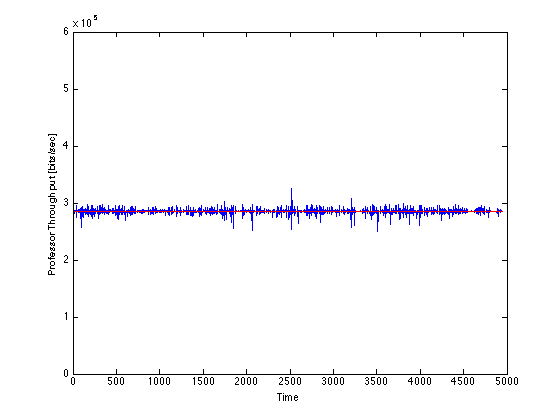
\includegraphics[width=\textwidth]{../Get_Simulation_Parameters/long_simulation_5000sec.png}
				\caption{Throughput over $5000\text{s}$}
				\label{fig:5000s}
			\end{figure}
			
			Our approach to this problem looks like this:
			
			We want to find a simulation time $m$ so that if we went through the throughput depicted in figure \ref{fig:5000s} and sliced it into time intervals of length $m$ - in a sliding window-like manner, and then averaged the throughput values inside the sliding windows, we want these means to be relatively close to each other. This would mean that our $m$ is large enough so that it does not matter much which sliding window we took, the result would be more or less the same. This is equivalent to looking at the variance of these mean values. We applied this procedure on the data from the $5000\text{s}$ run for all $m\in\{250\text{s},\, 350\text{s},\, 500\text{s},\, 750\text{s},\, 1000\text{s}\}$. The result can be seen in figure \ref{fig:relativevariance}.
			
			\begin{figure}[H]
				\center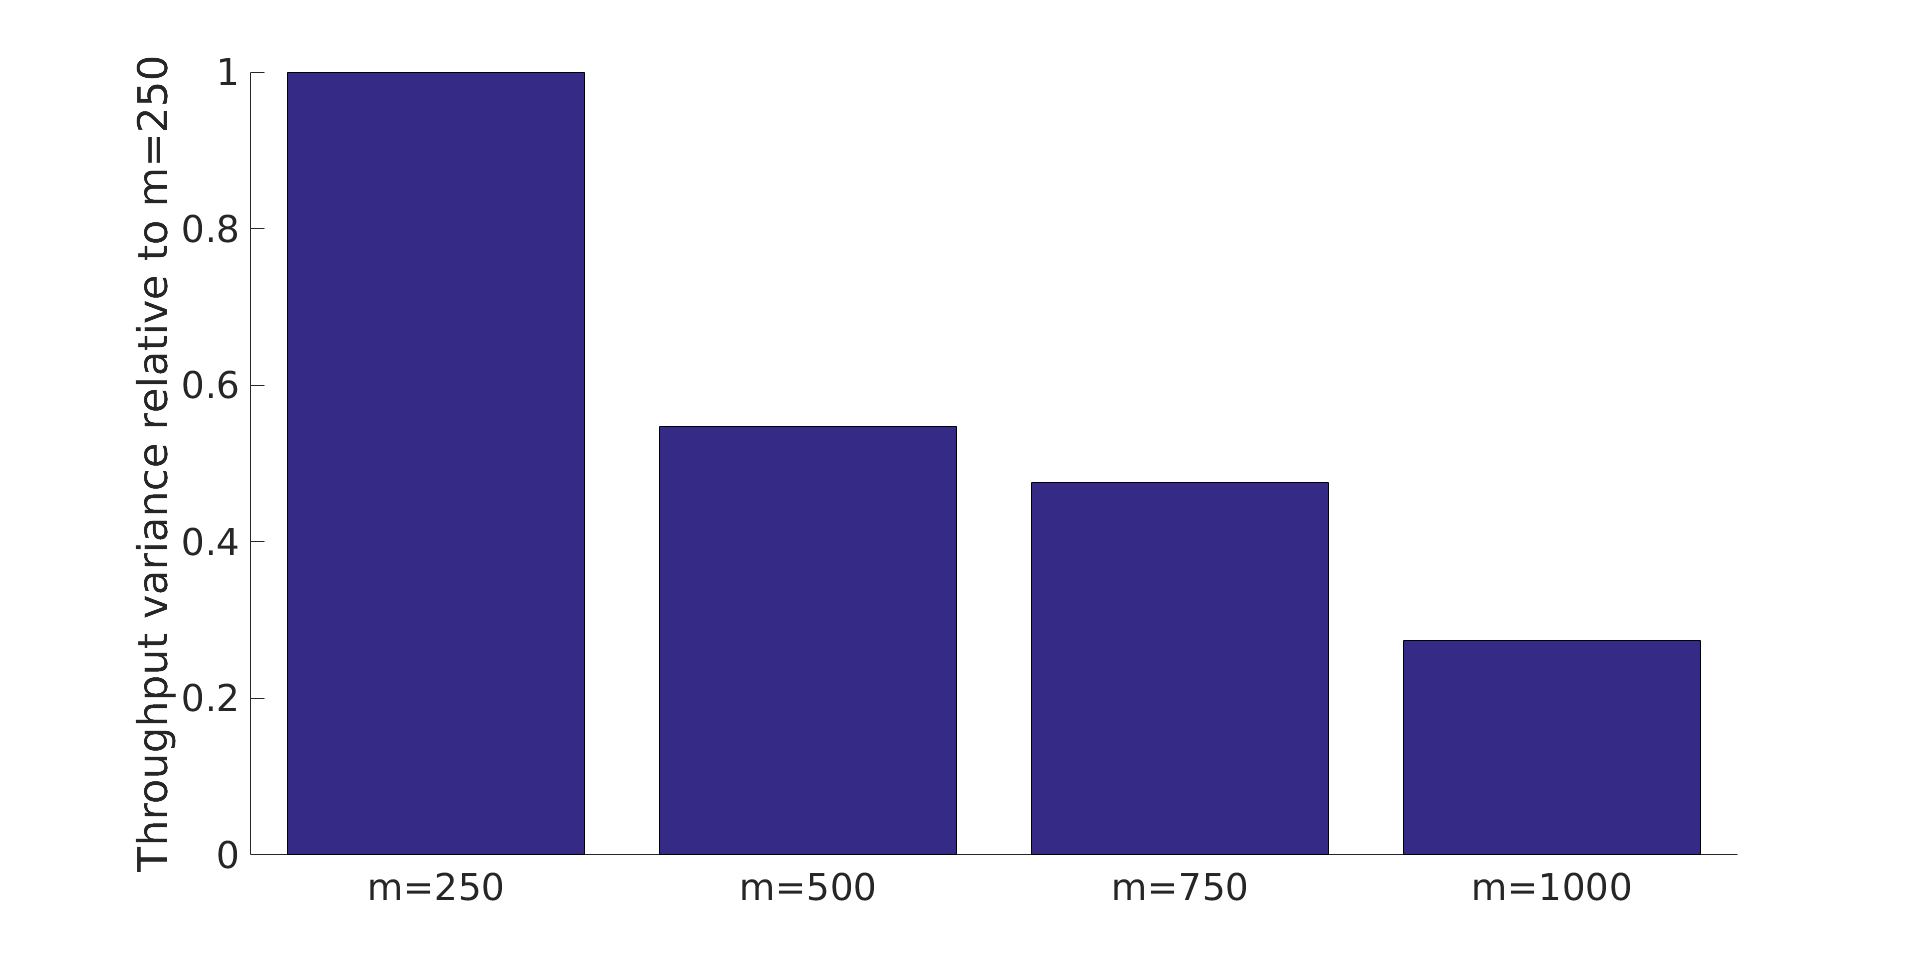
\includegraphics[width=\textwidth]{../Get_Simulation_Parameters/relative_variance.png}
				\caption{Relative variance of the throughput}
				\label{fig:relativevariance}
			\end{figure}
			
			One can observe that doubling $m$ from $m=250\text{s}$ to $m=500\text{s}$ roughly halves the variance. Increasing it further greatly increases the time required to run these simulations while gaining relatively little.
			
			This led us to the decision of setting the simulation time $m=500\text{s}$.
			
			\item[Number of Repetitions] As simulations rely on random events and those build upon pseudo-random numbers that we generate, it is important to run each and every simulation several times with new seeds for the random number generators in order to cover a meaningful number of possibilities with the goal of approximating real world behavior. 
			
			Each run's performance is recorded and denoted as a \emph{sample}. Following the \emph{Central Limit Theorem} we can assume a sample mean to stem from a \emph{Normal distribution}. 
			
			A sample mean estimate
			\[\mu_m=\frac{1}{m}\sum^m_{j=1}y_j\]
			where $m=\text{number of samples}$
			\\and $y_i=\text{i\textsuperscript{th} sample}$
			\\has a confidence interval of
			\[\mu_m-\frac{z\cdot \sigma}{\sqrt{m}}\leq \mu \leq \mu_m+\frac{z\cdot \sigma}{\sqrt{m}}\]
			where $\sigma=\text{Normal distribution's variance}$
			\\and $z$ is found using a Normal distribution's table using the required level of confidence $1-\alpha$, $\alpha\in [0,1]$.
			
			So apparently the confidence interval depends on $\frac{1}{\sqrt{m}}$, which looks like this:
			
			\begin{figure}[H]
				\center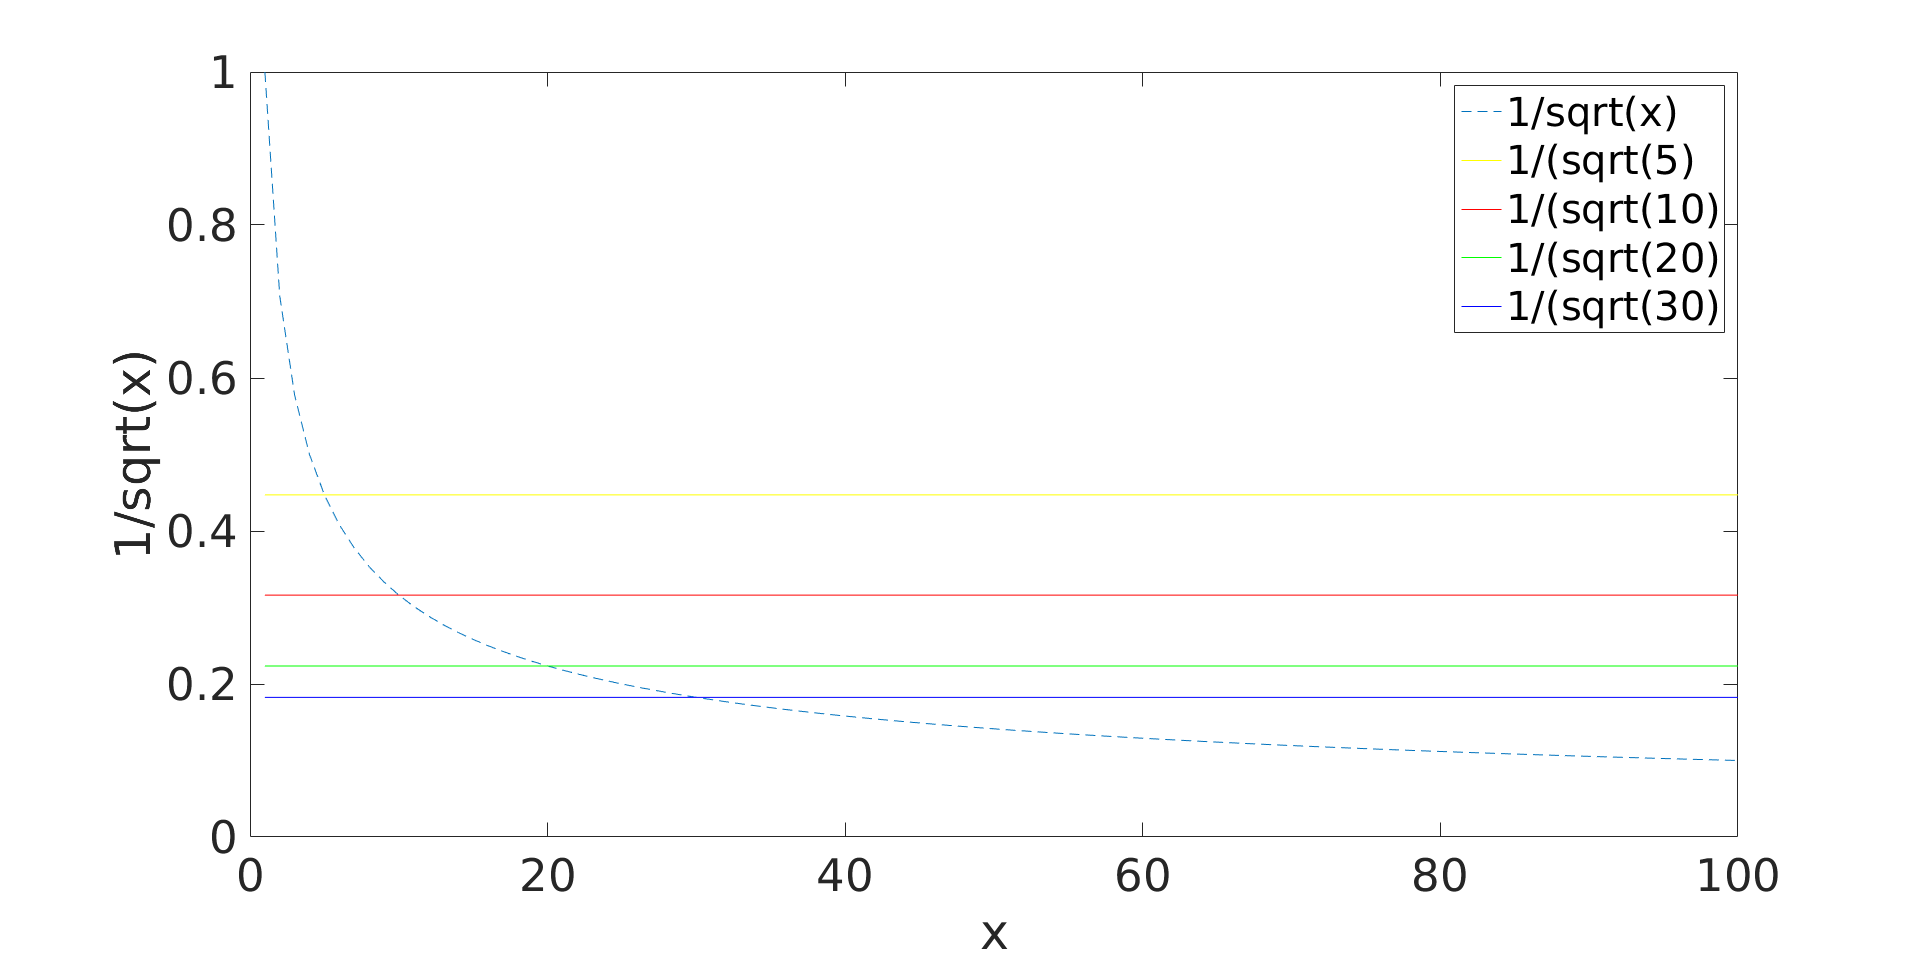
\includegraphics[width=\textwidth]{../Get_Simulation_Parameters/Number_Of_Runs.png}
				\caption{Behavior of $\frac{1}{\sqrt{x}}$}
				\label{fig:numberofruns}
			\end{figure}	
			
			In general it should hold that the more repetitions your simulation goes through, the closer its behavior gets to real world conditions. But as with many things, we want to find a good balance between \emph{correctness} and the \emph{required effort}, or a good efficiency in other words. From investigating figure \ref{fig:numberofruns} we concluded that setting $m=20$ seems like a good trade-off as at that point increasing $m>20$ further does not yield much better results anymore, relative to values of $m<20$ where performance gains are more significant.
			
			
			\item[Number of students] As the number of students is variable we simulated for a number of values, narrowing down the maximum number of students that could be supported when taking all requirements into account.
			
			
			\item[CCTV Camera] It was communicated to us that turning off the CCTV camera at the remote building location is an option. Thus we simulated every scenario once with the camera \emph{on} and once with it being \emph{off}.
		\end{description}		

\end{document}
